\section{Results and Performance Analysis}

To showcase the capabilities of our method, we applied it to three different mesoscale molecular scenes. 
For the rendering, we used cellVIEW \cite{muzic15}, a tool designed to efficiently render large molecular scenes on the GPU and is implemented in Unity3D. 
The different datasets have been generated by the domain experts with cellPACK \cite{cellpack}, a modeling tool for procedural generation of large biomolecular structures.
cellPACK summarizes and incorporates the most recent knowledge obtained from structural biology and system biology to generate comprehensive mesoscale models. 
Based on experimentally obtained data (such as proteins structure, concentration and spatial distribution), the tool is able to generate entire models of viruses and cells via a packing method based on collision constraints.

%The results of the packing with cellPACK is stored in a file and loaded in cellVIEW afterwards.  
%The file generated by cellPACK contains the description of the scene, namely, position, rotation and type of each individual instances.
%In order the load and display the scene, cellVIEW reads the instances information from the file and uploads it on the GPU memory thus allowing fast read accesses from the rendering pipeline.

\begin{figure*}[t]
\centering
\subfloat[]{\label{fig:res:gh3}\includegraphics[width=0.33\linewidth]{figures/res-gh3.eps}}
\subfloat[]{\label{fig:res:myco}\includegraphics[width=0.26\linewidth]{figures/mycoplasma.eps}}
\subfloat[]{\label{fig:res:eq}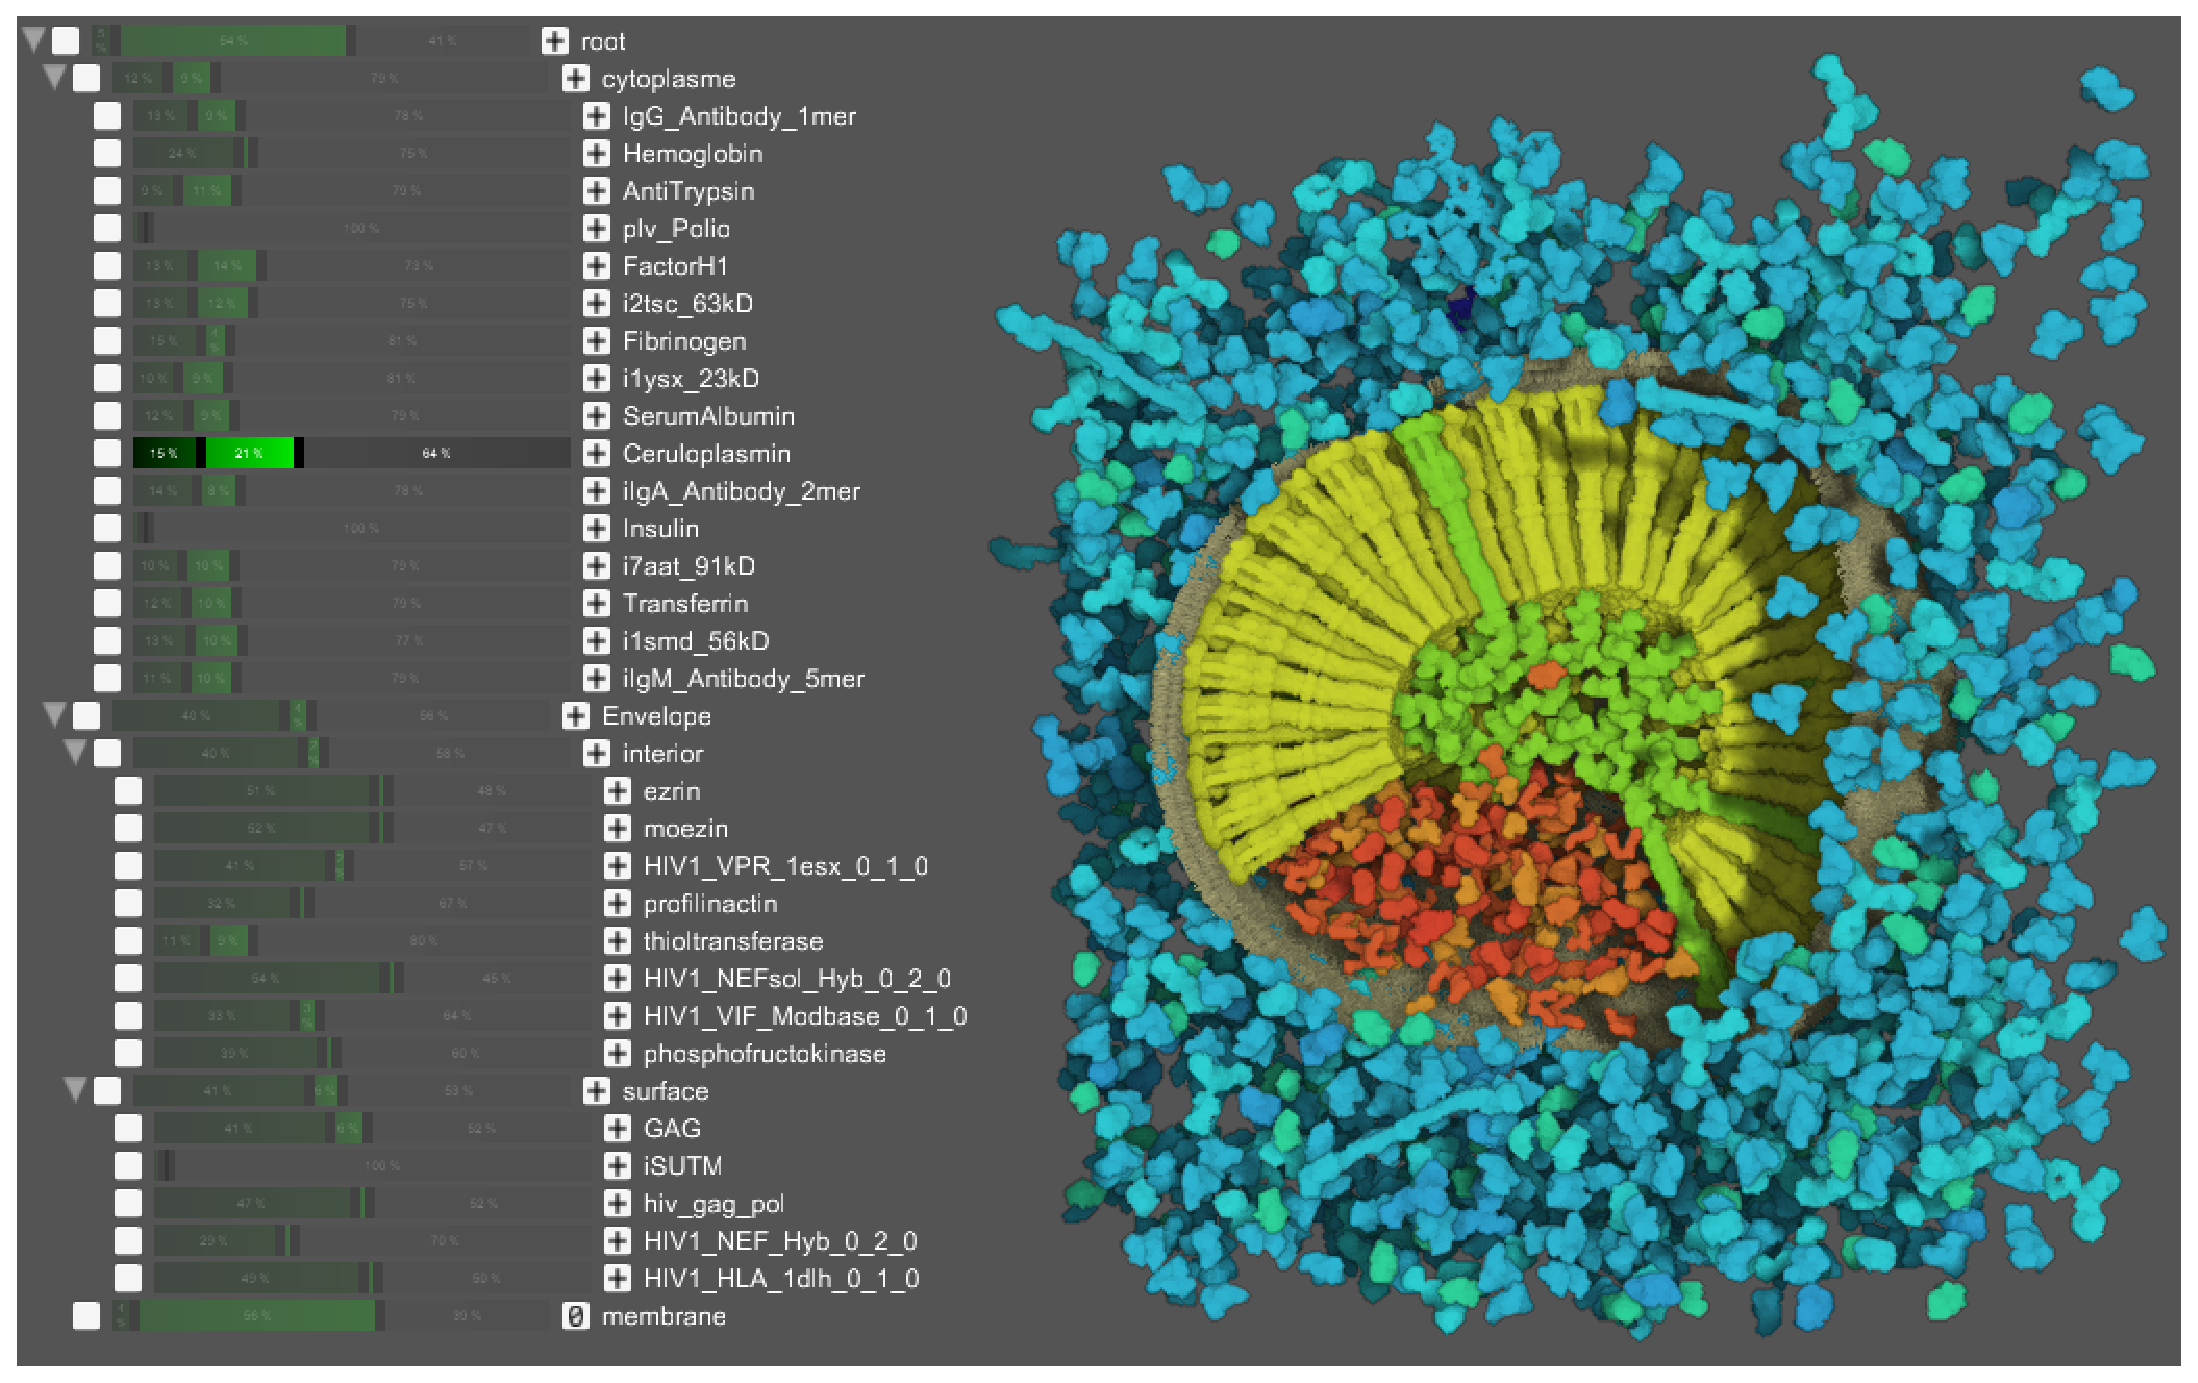
\includegraphics[width=0.4\linewidth]{figures/eq-s.eps}}
\caption{\label{fig:res:res}
(a) Mature HIV in blood serum. A clipping plane with below the dataset with a falloff function is used to gradually change the concentration of the blood serum molecules.
(b) Mycoplasma mycoides with ribosomes (blue) shown. 
(c) Internal structures of a immature HIV model are shown by several clipping objects. On the left, the visibility equalizer is shown.}
\vspace{-3mm}
\end{figure*}

The first dataset is a model of an HIV particle in blood serum that contains 20502 instances of 45 different protein types and 215559 instances of lipid molecules.
In Figure \ref{fig:res:gh3}, we show an example of a single clipping plane used to reduce the concentration of the blood serum molecules, so that the HIV proteins are visible. 
However, to avoid misleading the viewer about the actual concentration of the blood molecules, we render clipped proteins with a ghosting effect. 
This communicate true information about the concentration, while reducing visual clutter caused by the dense arrangement blood serum proteins.
Figure \ref{fig:teaser} shows sequential step for production a comprehensible cut-away illustration with the HIV dataset.

The second dataset is a model of \emph{Mycoplasma mycoides} that contains 5380 proteins of 22 different types. 
Figure \ref{fig:res:myco} shows how fuzzy-clipping is used to reduce visual clutter to illustrate the positions of the ribosomes (shown in blue) within the cell.

The third dataset, shown in Figure \ref{fig:res:eq} is a model of an immature HIV which contains 1081 instances of 13 different protein types. 
Here, we applied several clipping objects to reveal the internal structure of the virus. 
The blood serum (blue) has been preserved around the particle using the fuzzy clipping to illustrate how it encloses the HIV particle. 
The visibility equalizer is displayed as well, showing the ratios of visible and clipped instances of the individual molecular ingredients. 
The white boxes to the left of each stacked bar are used to mark the given ingredient or compartment as focus.

\begin{figure}[b]
\vspace{-4mm}
\centering
\includegraphics[width=0.89\linewidth]{figures/res-islands.eps}
\caption{\label{fig:res:islands}
HIV clipped with a plane. 
%Envelope proteins (blue) are reintroduced in the scene. 
Contextual anchoring is used to indicate the proximity of envelope proteins (dark blue) with the lipid membrane (grey)
The dark spots represent shadows projected into interior proteins.}
\end{figure}

Figure \ref{fig:res:islands} shows the mature HIV dataset clipped with a single plane. 
The contextual anchoring is applied to reintroduce parts of the clipped membrane (grey) around the envelope proteins (blue).

%\begin{figure}[t]
%\centering
%\subfloat[]{\label{fig:res:gh0}\includegraphics[width=0.5\linewidth]{figures/res-gh0.eps}}
%\subfloat[]{\label{fig:res:gh1}\includegraphics[width=0.5\linewidth]{figures/res-gh1.eps}}

%\subfloat[]{\label{fig:res:gh2}\includegraphics[width=0.5\linewidth]{figures/res-gh2.eps}}
%\subfloat[]{\label{fig:res:gh3}\includegraphics[width=0.5\linewidth]{figures/res-gh3.eps}}
%\caption{\label{fig:res:gh}The cutaway molecules are indicated through the ghosting effect. (a) Part of the scene is removed by a clipping plane. (b) The amount of cutaway molecules has been decreased through the fuzzy clipping, which caused some of the cutaway molecules to be reintroduced into the scene. (c) The blood serum (red molecules) are removed by fuzzy clipping in the entire dataset. (d) A falloff function is used to gradually change the influence of the fuzzy clipping.}
%\end{figure}
 
%Figure \ref{fig:res:gh} illustrates that this can be done in different ways according to the vision of the artist.

The visibility equalizer is designed to limit the computational overhead in order to offer a fast and responsive user experience.
To demonstrate the responsiveness of our method, we measured the computation time for the object-space clipping, view-space clipping and 2D distance transform, respectively.
The application was running on a machine equipped with an Intel Core i7-3930 CPU 3.20 GHz machine coupled with a GeForce GTX Titan X graphics card with 12GB of video RAM. 
The computation of the object-space clipping, compared to the rendering task performed by cellVIEW, is very lightweight and does not impact the overall performance too much. 
It took \textbf{0.3 milliseconds} to evaluate the 236061 instances of the HIV + blood dataset without clipping any of them.
It took \textbf{0.5 milliseconds} in total to slice the dataset in half and \textbf{0.6 milliseconds} to clip it entirely.
The increasing cost corresponds to the writing operations to the video memory, which are performed when an instance is clipped.
It is important to mention that neither the shape of the clipping object nor the number of clipping objects have a meaningful influence on the performance.

The view-space clipping, however, requires more computational work that could impact the responsiveness. 
%Therefore, a good strategy is to limit the number of view-space clipping objects, especially for very large scenes with up to several million instances. 
Indeed, for computing occlusion queries, occluders and occludees must be additionally rendered, which adds extra work to the rendering pipeline. 
For this reason, only the bounding spheres of the molecules are rendered instead of their entire structures, which may consist of hundreds or thousands of spheres, in order to guarantee a minimal computational overhead. 
We measured \textbf{0.07 milliseconds} for rendering the depth-stencil mask with 12142 instances (HIV proteins), and \textbf{0.57 milliseconds} for the computation of the 223919 occlusion queries corresponding to the remaining objects of the scene (blood proteins + lipid residues).
Additionally, the 2D distance transform that is needed for the aperture effect also requires additional computation.
It took \textbf{0.15 milliseconds} for computing the distance transform of the previous depth-stencil mask at a resolution of 512 by 512 pixels.
Unlike object-space clipping, the view-space clipping computation cost will keep increasing with additional operations.
Therefore it is a good strategy to keep a low number of view-space clipping objects, especially with very large scenes.

%\begin{figure}[t]
% \centering
%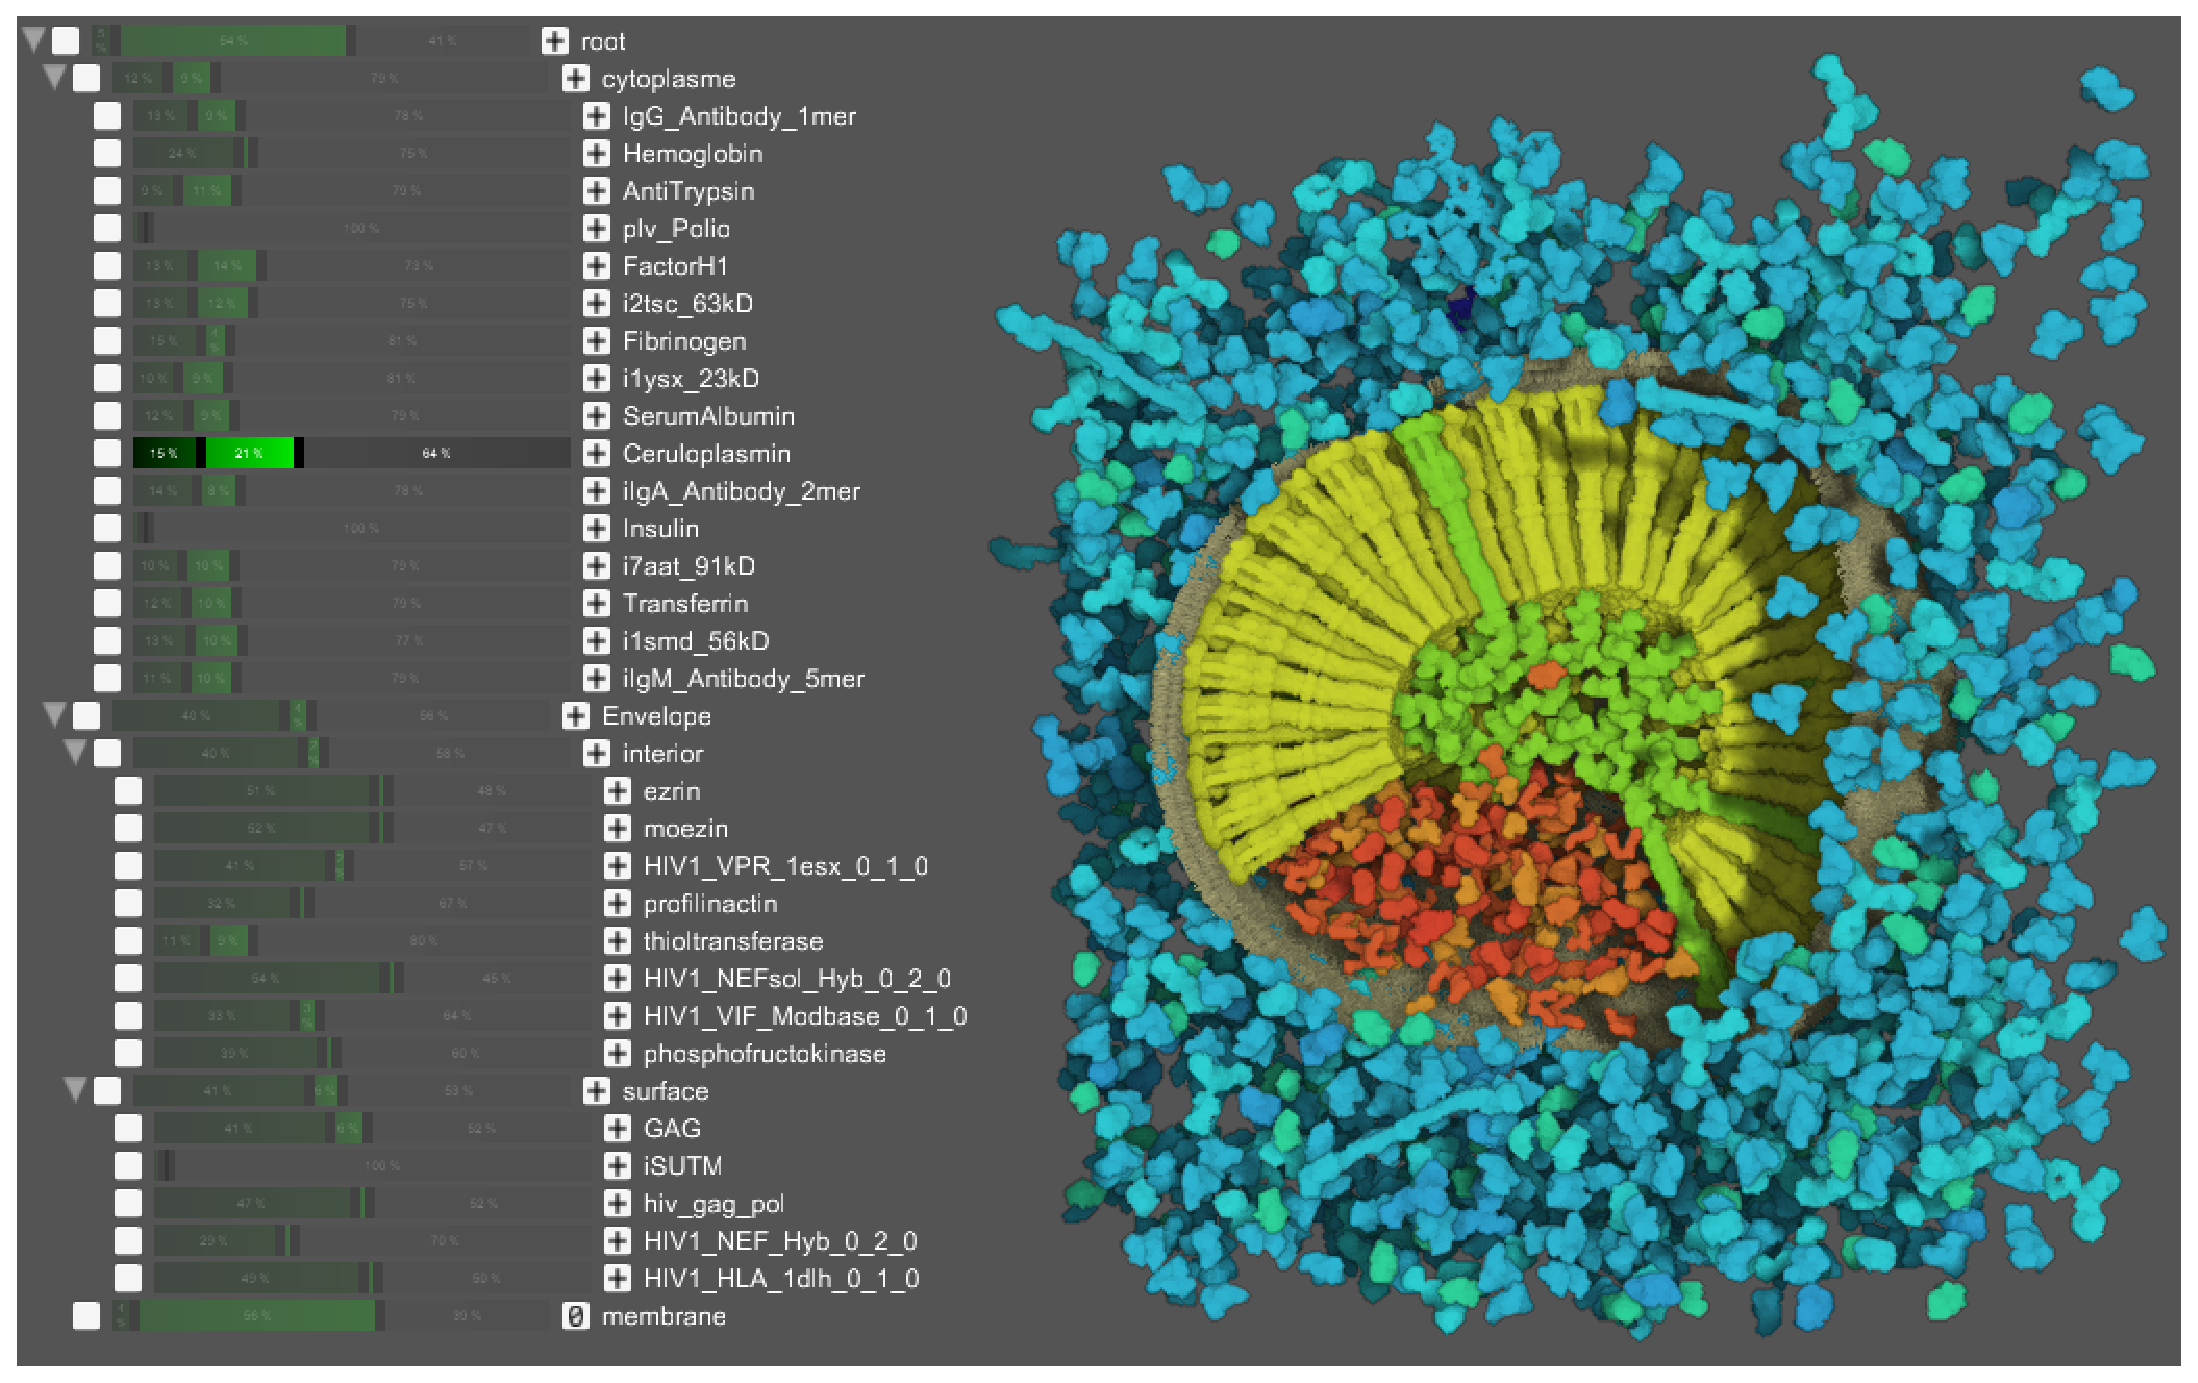
\includegraphics[width=\linewidth]{figures/eq-s.eps} %\caption{\label{fig:res:eq}Mature HIV.}
%\end{figure}


%\begin{figure}[t]
%\centering
%\subfloat[]{\label{fig:res:vsc0}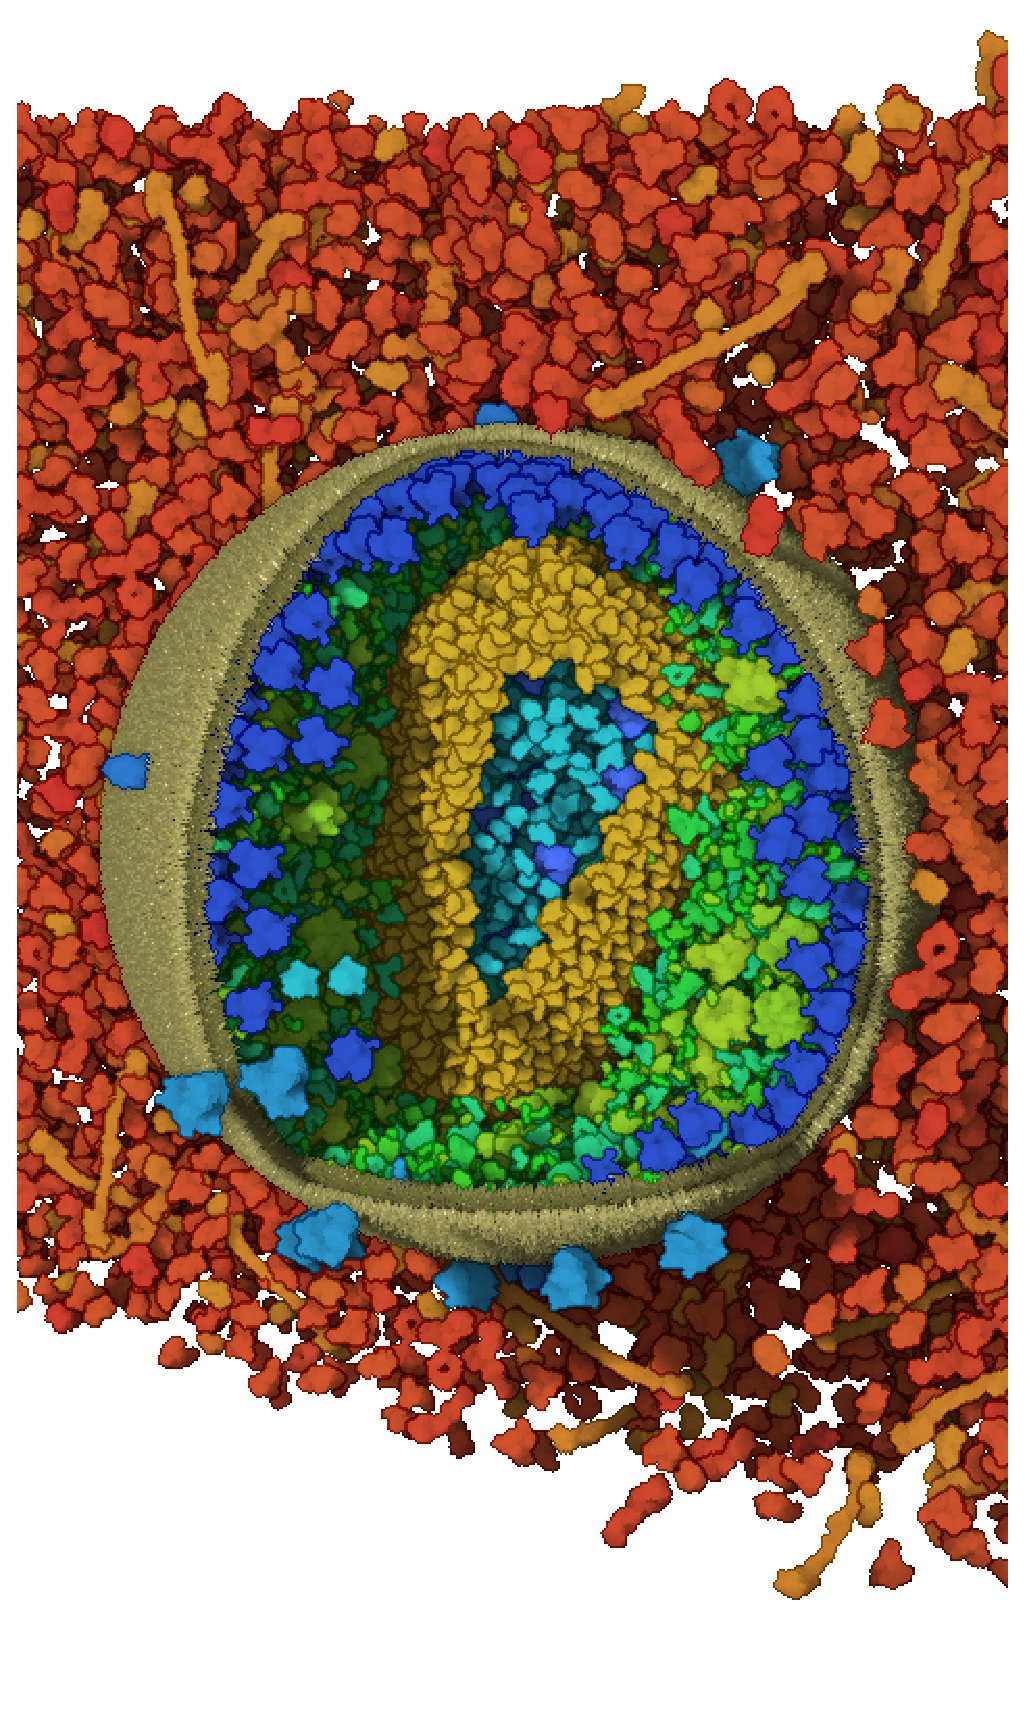
\includegraphics[width=0.245\linewidth]{figures/res-vsc0.eps}}
%\hfill
%\subfloat[]{\label{fig:res:vsc1}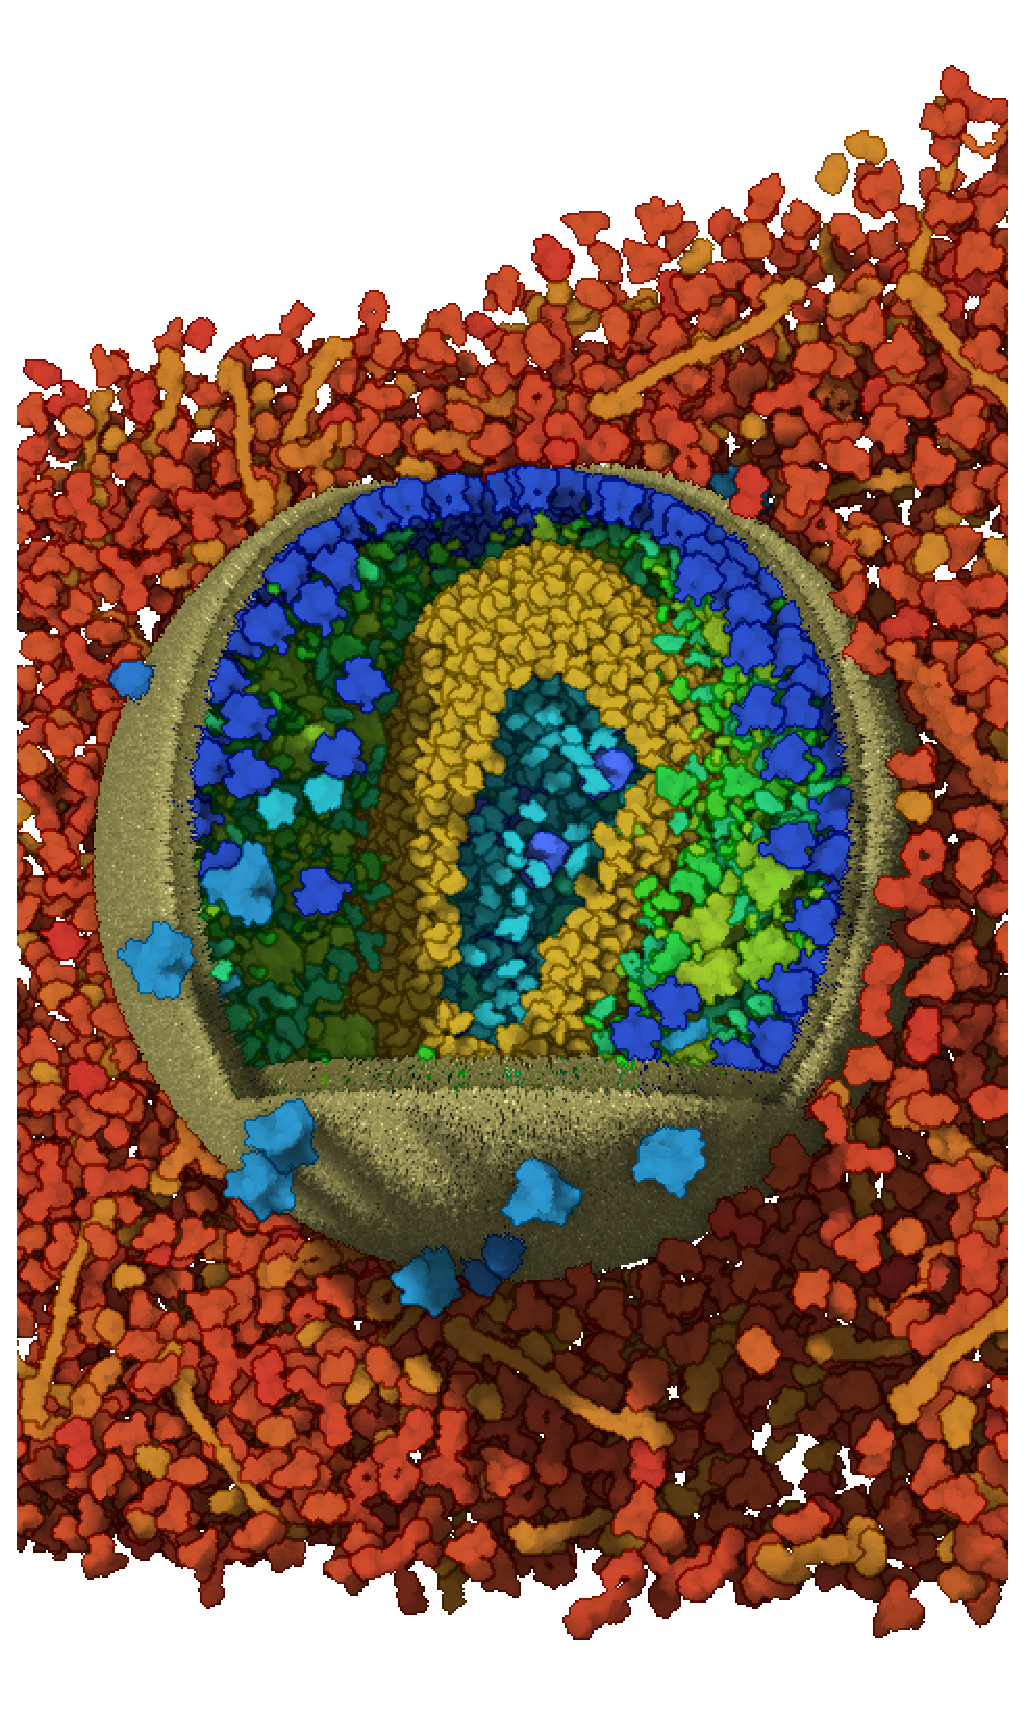
\includegraphics[width=0.245\linewidth]{figures/res-vsc1.eps}}
%\hfill
%\subfloat[]{\label{fig:res:vsc2}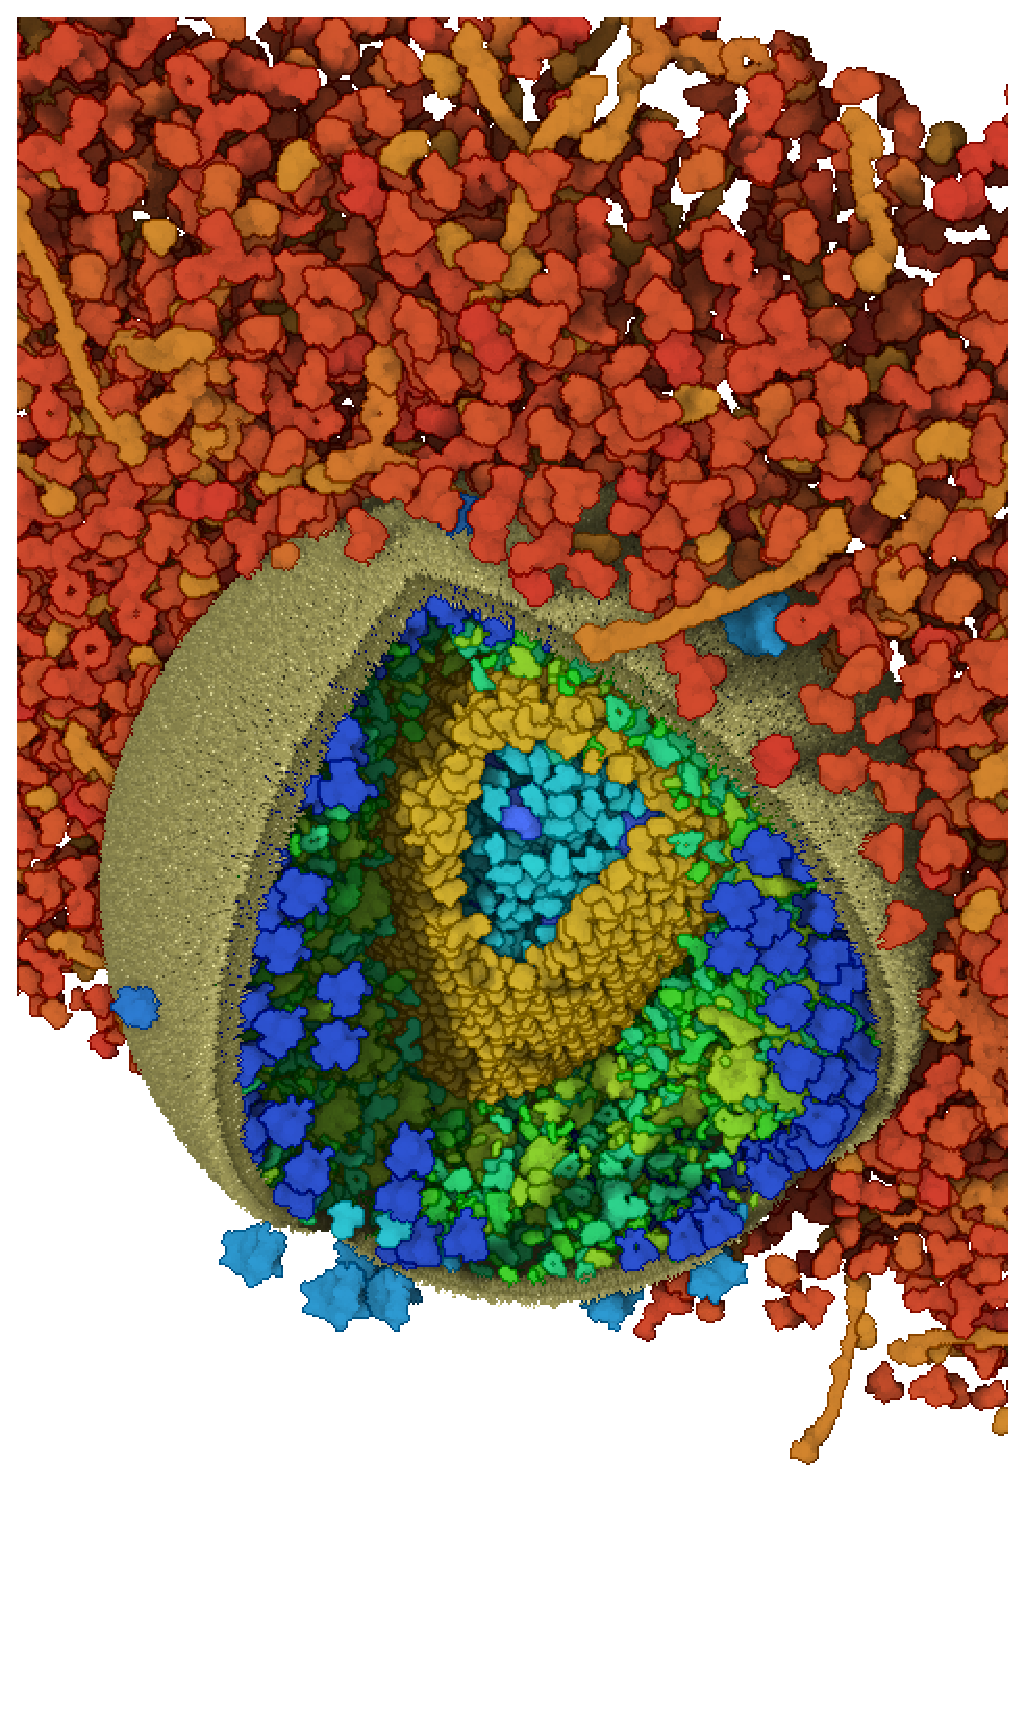
\includegraphics[width=0.245\linewidth]{figures/res-vsc2.eps}}
%\hfill
%\subfloat[]{\label{fig:res:vsc3}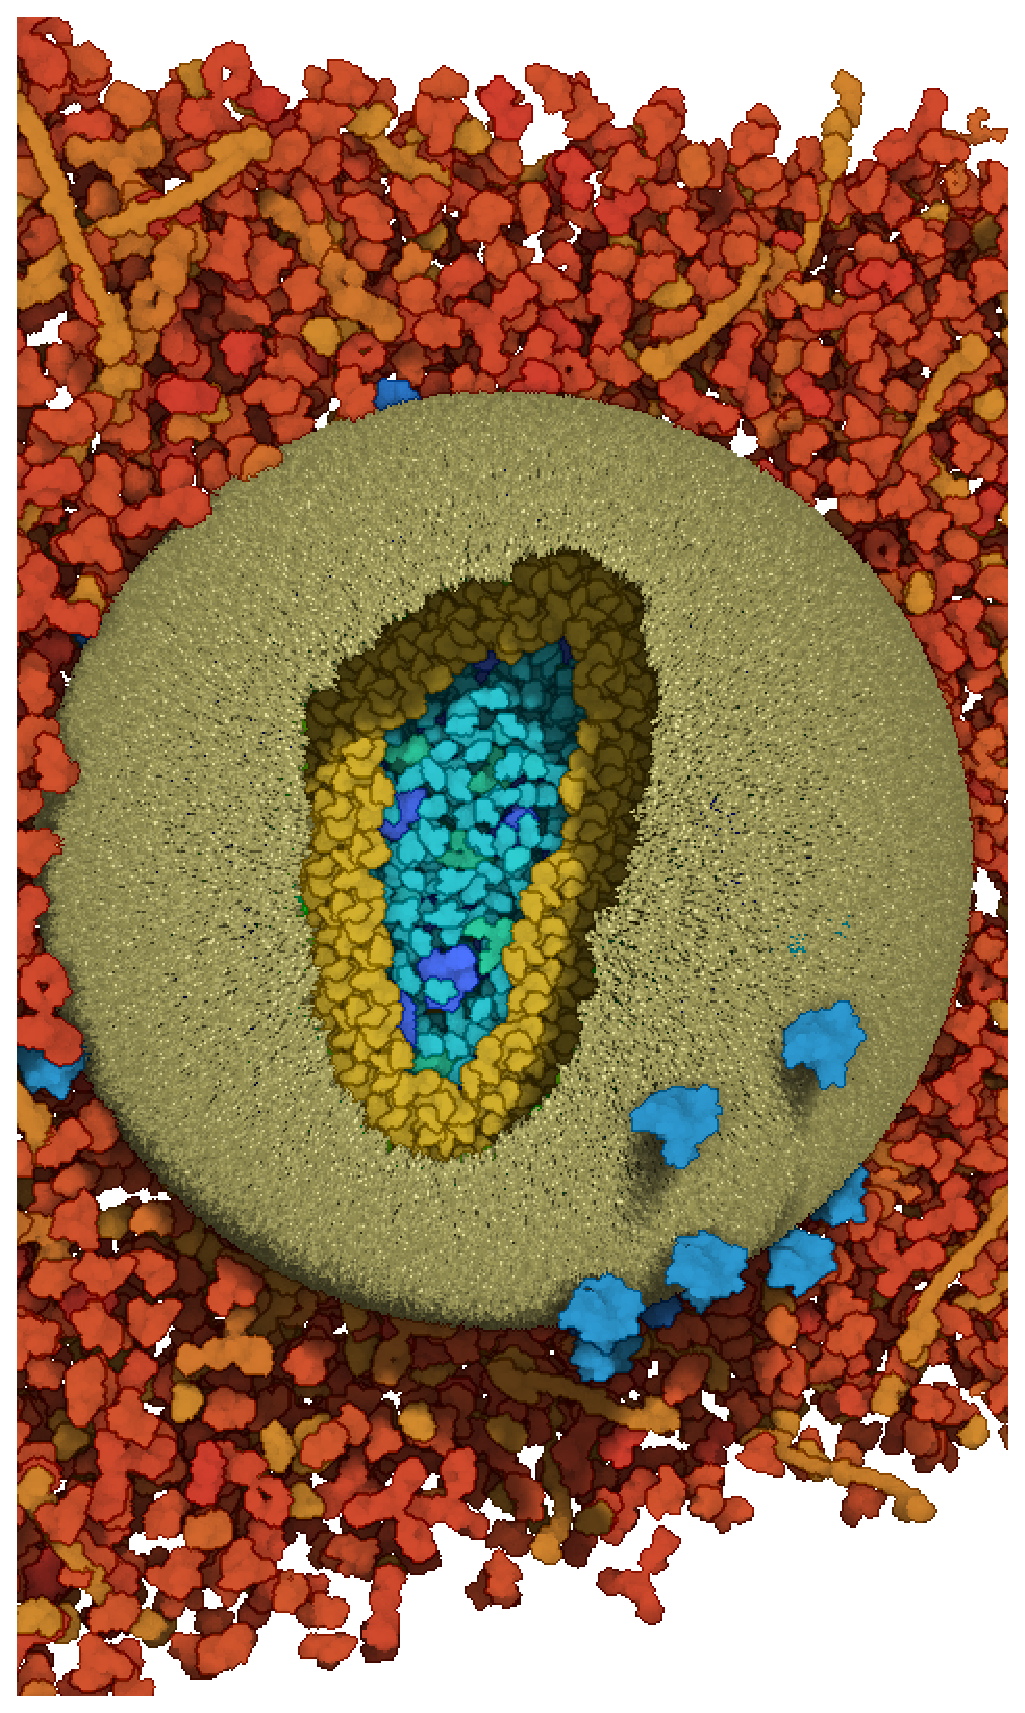
\includegraphics[width=0.245\linewidth]{figures/res-vsc3.eps}}
%\caption{\label{fig:res:gh}View-space clipping.}
%\end{figure}

%\begin{figure*}[t]
%\centering

%\subfloat[]{\label{fig:res:w0}\includegraphics[width=0.25\linewidth]{figures/res-w0.eps}}
%\subfloat[]{\label{fig:res:w1}\includegraphics[width=0.25\linewidth]{figures/res-w1.eps}}
%\subfloat[]{\label{fig:res:w2}\includegraphics[width=0.25\linewidth]{figures/res-w2.eps}}
%\subfloat[]{\label{fig:res:w3}\includegraphics[width=0.25\linewidth]{figures/res-w3.eps}}

%\subfloat[]{\label{fig:res:w4}\includegraphics[width=0.25\linewidth]{figures/res-w4.eps}}
%\subfloat[]{\label{fig:res:w5}\includegraphics[width=0.25\linewidth]{figures/res-w5.eps}}
%\subfloat[]{\label{fig:res:w6}\includegraphics[width=0.25\linewidth]{figures/res-w6.eps}}
%\subfloat[]{\label{fig:res:w7}\includegraphics[width=0.25\linewidth]{figures/res-w7.eps}}
%\caption{\label{fig:res:w}W.}
%\end{figure*}

%\begin{figure}[t]
% \centering
% \includegraphics[width=\linewidth]{figures/results01.eps}
% \caption{\label{fig:results01}An illustration of the HIV virus in the %blood serum utilizing cutaways created with our approach.}
%\end{figure}
